\documentclass[11pt]{article}
\usepackage[utf8]{inputenc}
\usepackage[hmargin={2cm,2cm}, vmargin={2cm,2cm}]{geometry}
\usepackage{amsmath,amssymb,amsfonts}
\usepackage{steinmetz}
\usepackage[colorlinks=blue,hidelinks]{hyperref}
\usepackage{fancyhdr}
\usepackage{graphicx}
\usepackage{xcolor}
\usepackage{tcolorbox}
\usepackage{multirow}
\usepackage{multicol}
\usepackage{float}
\usepackage[rflt]{floatflt}
\usepackage{tikz}
\usepackage{pgfplots}
\usepackage{pdfpages}
\usepackage{tikz-page}
\usepackage{circuitikz}
\usepackage{siunitx}
\usepackage{caption}
\usepackage{listings}
\usepackage[explicit]{titlesec}
\usepackage{soul}
\usepackage{datatool}
\usepackage{tabularx}
\usetikzlibrary{shapes.geometric, arrows}

% Start of preamble

% Block diagrams
\tikzstyle{startstop} = [rectangle, rounded corners, minimum width=3cm, minimum height=1cm,text centered, draw=black, fill=red!50!blue!40]
\tikzstyle{arrow} = [thick,->,>=stealth]

% For units
\newcommand{\volt}{\si{\volt}}
\newcommand{\ampere}{\si{\ampere}}
\newcommand{\kohm}{\si{\killo\ohm}}
\newcommand{\ohm}{\si{\ohm}}
\newcommand{\watt}{\si{\watt}}
\newcommand{\hour}{\si{\hour}}


% End of preamble

\begin{document}
    \thispagestyle{empty}
\newgeometry{hmargin={20mm,20mm}, vmargin={20mm,20mm}}
\tikz[remember picture, overlay]{
    \draw[blue, line width= 4mm](current page.south west) rectangle (current page.north east);
}

\begin{center}

    \begin{center}
        \Large{Central University of Venezuela}\\
        \Large{Faculty of Engineering}\\
        \Large{School of Electrical Engineering}\\
        \Large{Department of Electronics, Computing and Control}
    \end{center}
    \vfill

    \LARGE{\textbf{Project}}\\
    \vspace{0.25cm}
    
\begin{tikzpicture}[overlay]
        \rotatebox{5}{\fill[blue!65] (0,-2.3) rectangle (17,1);}
    \end{tikzpicture}
    \huge{\textbf{\color{white} Battery Charging System Design with Current Control}}\\
    \vfill

    \LARGE{\textbf{Teaching:}}\\
    \vspace{0.1cm}
    \Large{Alonso, Jose}\\
    \vspace{1cm}


    \LARGE{\textbf{Estudent:}}\\
    \vspace{0.1cm}
    \Large{Br. Lopez, Jose}\\
    \vspace{0.07cm}

    \vfill
    
\begin{tikzpicture}[overlay]
        \rotatebox{-4.5}{\fill[green!45] (0,0.5) rectangle (2.3,-0.1);}
    \end{tikzpicture}
    \textsc{\normalsize{2025/04/02}}
\end{center} 
    \tableofcontents
    \restoregeometry
    % For sections, subsections and subsubsections
    \definecolor{titleblue}{HTML}{4a7aa4}
    \newbox\TitleUnderlineTestBox
    \newcommand*\TitleUnderline[1]
      {%
        \bgroup
        \setbox\TitleUnderlineTestBox\hbox{\colorbox{titleblue}\strut}%
        \setul{\dimexpr\dp\TitleUnderlineTestBox-.3ex\relax}{.3ex}%
        \ul{#1}%
        \egroup
      }
    \newcommand*\SectionNumberBox[1]
      {%
        \colorbox{titleblue}
          {%
            \makebox[2.5em][c]
              {%
                \color{white}%
                \strut
                \csname the#1\endcsname
              }%
          }%
        \TitleUnderline{\ \ \ }%
      }
      \titleformat{\section}
      {\LARGE\bfseries\sffamily\color{titleblue}}
      {\SectionNumberBox{section}}
      {0pt}
      {\TitleUnderline{#1}}
      
    \titleformat{\subsection}
      {\Large\bfseries\sffamily\color{titleblue}}
      {\SectionNumberBox{subsection}}
      {0pt}
      {\TitleUnderline{#1}}
      
    \titleformat{\subsubsection}
      {\large\bfseries\sffamily\color{titleblue}}
      {\SectionNumberBox{subsubsection}}
      {0pt}
      {\TitleUnderline{#1}}
      
    \section{Introduction}

Today, lithium-ion batteries have become a fundamental part of our daily lives, powering everything from smartphones to electric vehicles and renewable energy storage systems. As the demand for portable and sustainable devices continues to grow, the need to develop efficient and safe battery charging systems becomes increasingly critical.\\

However, charging batteries presents several challenges, including voltage and current management, which, if not properly controlled, can result in battery degradation, overheating, or even fire risks. Therefore, it is essential to have a system that not only efficiently charges batteries but also continuously monitors their condition.\\

This project aims to design a lithium-ion battery charging system that includes current and voltage control, ensuring a safe charging process and extending battery life. Through the development of this system, we hope to learn about the integration of electronic components, the importance of charge control, and best practices for circuit design.\\

Furthermore, the proposed system has practical applications in diverse areas, including mobile device charging stations, sustainable energy systems, and electric vehicles, underscoring the relevance of this project in a global context. 
    \section{Theoretical Framework}

\subsection{Battery}

It is an electrochemical device that stores chemical energy and converts it into direct current (DC) electrical energy when required. Its basic operation is as follows:

\begin{itemize}
    \item A battery consists of one or more electrochemical cells. Each cell contains a positive electrode (cathode), a negative electrode (anode), and an electrolyte.
    \item Chemical reactions between the electrodes and the electrolyte generate a flow of electrons, which produces electric current.
\end{itemize}

\subsubsection{Types of Batteries}

\begin{itemize}
    \item \textbf{Primary batteries (not rechargeable)}: Designed for single use and then discarded. Examples: alkaline batteries, primary lithium batteries.
    \item \textbf{Secondary batteries (rechargeable)}: They can be charged and discharged repeatedly. Examples: lead-acid, lithium-ion, and nickel-cadmium batteries.
\end{itemize}

\subsubsection{Parameters}

Like every device, it has its parameters or system characteristics that must be monitored:

\begin{itemize}
    \item \textbf{Voltage:} The electric potential difference between the battery's terminals.
    \item \textbf{Capacity:} The amount of electrical charge a battery can store, usually measured in ampere-hours ($\ampere\cdot\hour$).
    \item \textbf{Discharge current:} The amount of current a battery can safely supply.
    \item \textbf{Internal resistance:} The resistance to the flow of current within the battery.
    \item \textbf{Life cycle:} The number of charge and discharge cycles a battery can withstand before its performance decreases.
\end{itemize}

\subsubsection{How can they be charged?}

As is commonly known, batteries must be charged and discharged using Direct Current (DC), and for this, there are charging methods, which are as follows:

\begin{itemize}
    \item \textbf{Constant Current (CC) Charging:}
    \begin{itemize}
      \item A constant current is applied to the battery until it reaches a certain voltage.
      \item This method involves supplying a constant current to the battery during most of the charging process.
      \item It is useful for charging batteries that are deeply discharged, as it allows for a quick initial charge.
      \item If constant current charging is continued once the battery is almost full, overcharging can occur and damage the battery.
    \end{itemize}
    \item \textbf{Constant Voltage (CV) Charging:}
    \begin{itemize}
      \item A constant voltage is maintained across the battery while the current gradually decreases.
      \item A constant voltage is maintained at the battery terminals while the charging current gradually decreases as the battery charges.
      \item It is a safer method than constant current charging, as the current automatically decreases as the battery approaches its maximum capacity.
    \end{itemize}
    \item \textbf{CC/CV Charging:}
    \begin{itemize}
      \item A combination of the two previous methods, common in lithium-ion batteries.
      \item Charging begins with a constant current until the battery reaches a certain voltage. Then, the charger switches to constant voltage, and the current gradually decreases until the battery is fully charged.
    \end{itemize}
\end{itemize}

Obviously, other considerations are attributed to all this, such as temperature, overcharging, deep discharge, and suitable chargers. The constant current charging method has other types of charging: \textbf{Pulse charging}\footnote{This method involves applying current pulses to the battery, followed by rest periods.}, and \textbf{Trickle charging}\footnote{This method involves applying a small constant current to the battery after it has been fully charged to maintain it at its maximum capacity.}

\subsection{Operating Principle of a Solar Panel}

A solar panel is a device that transforms solar energy into electricity or heat. This is done through the \textbf{Photovoltaic Effect}. This is a physical phenomenon by which a semiconductor material (mostly silicon) generates an electric current when sunlight strikes it. When photons are absorbed by the material, it excites the electrons of the semiconductor, generating an electron-hole pair (a free electron and a positive hole). This causes the excited electrons to move towards the "N-layer"\footnote{This layer is doped with phosphorus, which gives it an excess of electrons (negative charge).} while the holes move to the "P-layer"\footnote{This layer is doped with boron, creating a shortage of electrons (positive charge).} due to the charge difference. This creates an electric field at the P-N junction (Intrinsic layer), generating an electric current (direct current).\\

The generated current flows to an external circuit that can be used to power electrical devices or charge batteries. To increase energy production, multiple cells are connected in series and parallel, forming a solar panel. There are factors that affect its performance:

\begin{itemize}
  \item \textbf{Sunlight intensity:} The higher the intensity, the greater the electricity generation.
  \item \textbf{Angle of incidence:} Efficiency is maximum when light strikes the panel perpendicularly.
  \item \textbf{Temperature:} Solar panels are less efficient at very high temperatures.
  \item \textbf{Shading:} Shadows on the panel significantly reduce its performance.
  \item \textbf{Material efficiency:} Depends on the type of photovoltaic cell (monocrystalline, polycrystalline, or thin-film).
\end{itemize}

\subsection{Operating Principle of a Voltage Regulator}

They are devices that maintain a constant output voltage, regardless of variations in the input voltage or the connected load. There are two main types of voltage regulators:

\begin{itemize}
  \item \textbf{Linear:} they dissipate excess energy as heat to maintain a constant voltage. They are simple but less efficient.
  \item \textbf{Switching:} they use a switch (transistor) that turns on and off at a high frequency to control the power sent to the load. They are more efficient than linear regulators, as they convert energy more effectively and generate less heat. They are implemented as Buck, Boost, or Buck-Boost converters.
\end{itemize}

\subsection{Operating Principle of a DC-DC Converter}

These are circuits that allow converting a DC input voltage into another output voltage, either of a higher or lower value. The most common types include:

\begin{itemize}
  \item \textbf{Buck converter:} reduces the input voltage to a lower level. It uses a switch (transistor) and an inductor to store energy. When the switch is closed, energy accumulates in the inductor. When it opens, the energy is transferred to the load.
  \item \textbf{Boost converter:} increases the input voltage to a higher level. It works similarly to the Buck, but the inductor is disconnected from the source and connected to the load, generating a higher voltage.
  \item \textbf{Buck-Boost converter:} can increase or decrease the input voltage as needed. It combines elements of the previous two.
\end{itemize}

\subsection{Operating Principle of a Current Sensor}

Current sensors measure the current flowing in a circuit and are commonly used in battery charging to monitor the state and efficiency of the charging process. The most common types include:

\begin{itemize}
  \item \textbf{Hall effect sensors:} measure current through an electromagnetic principle. A magnet is placed near a conductor, and the generated magnetic field causes a small voltage that is measured and translated into a current measurement. They are non-intrusive and allow measurements in circuits without needing to interrupt the current.
  \item \textbf{Shunt Resistors:} a known resistance is placed in series with the load. By measuring the voltage drop across this resistor, the current can be calculated using Ohm's Law (V = I * R). This method is simpler but intrusive.
\end{itemize}
    \section{Development}

The goal is to design a system that covers the entire process from energy acquisition to its final use, including a storage system (battery). A simple design for the whole system will be outlined, covering simulation, schematic design, PCB design (using the KiCad tool), among other software. The initial plan for this project is shown in the following block diagram in Figure \ref{Diagrama 1}:

\begin{figure}[H]
    \centering
    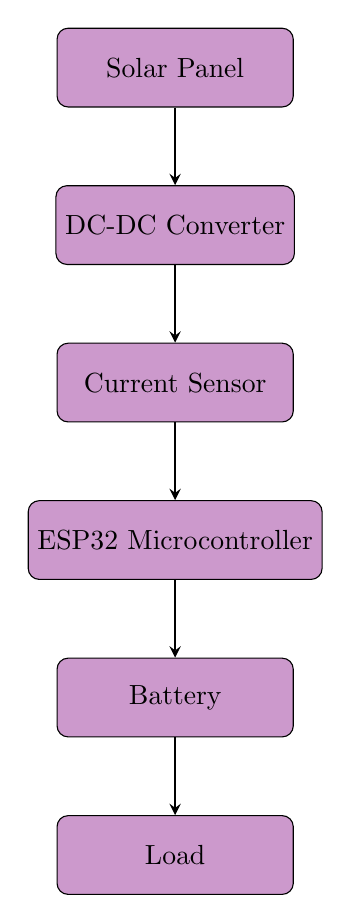
\begin{tikzpicture}[node distance=2cm]
        \node (Solarcell) [startstop] {Solar Panel};
        \node (Regulator) [startstop, below of = Solarcell] {DC-DC Converter};
        \node (CurrentSensor) [startstop,below of = Regulator] {Current Sensor};
        \node (Micro) [startstop,below of = CurrentSensor] {ESP32 Microcontroller};
        \node (Battery) [startstop,below of = Micro] {Battery};
        \node (Load) [startstop,below of = Battery] {Load};
          
        \draw[arrow] (Solarcell) -- (Regulator);
        \draw[arrow] (Regulator) -- (CurrentSensor);
        \draw[arrow] (CurrentSensor) -- (Micro);
        \draw[arrow] (Micro) -- (Battery);
        \draw[arrow] (Battery) -- (Load);
    \end{tikzpicture}
    \caption{Block diagram to follow}
    \label{Diagrama 1}
\end{figure}

\newpage
\subsection{Theoretical Calculations}
\label{DesaTeorico}

\subsubsection{Solar Panel}

Let's assume the following solar panel model, \textbf{RNG-100D}, for the theoretical calculations, and we will use a basic model following Figure \ref{ModelPanel}. The irradiance reaching the photodiode will be replaced by a DC current source, which we will then simulate.

\begin{figure}[H]
    \centering
    \begin{circuitikz}[american]\draw
        to[I, l=$I_{ph}$,name=fuente] ++(0,2) --++(2,0)coordinate(A) to[D,l=$D_{1}$, fill=black] ++(0,-2) coordinate(B) -| (fuente.west)
        (A)--++(2,0) coordinate(A1) to[D,l=$D_{2}$, fill=black] ++(0,-2) coordinate(B1) -| (B)
        (A1) --++(2,0) coordinate(A2) to[R,l=$R_{p}$] ++(0,-2) coordinate(B2) -| (B1)
        (A2) to[R,l=$R_{s}$] ++(2,0) to[short,-o] ++(0,0) node[label, color=blue, below]{$+$}
        (B2) --++(2,0) to[short,-o] ++(0,0) node[label, color=red, above]{$-$}
    ;\end{circuitikz}
    \caption{Basic model of a solar panel (Double Diode)}
    \label{ModelPanel}
\end{figure}

Where:

\begin{itemize}
  \item $I_{ph}$: Generated current.
  \item $R_{p}$: Parallel resistance (models leakage losses).
  \item $R_{s}$: Series resistance (models internal losses).
\end{itemize}

\begin{figure}[H]
    \centering
    \begin{minipage}[c]{0.30\textwidth}
        \begin{equation*}
            I_{ph} = G\cdot A \cdot \eta
        \end{equation*}
        Where:
        \begin{itemize}
          \item $G$: Solar irradiance [\watt/\si{\meter\squared}].
          \item $A$: Panel area [\si{\meter\squared}].
          \item $\eta$: Panel efficiency.
        \end{itemize}
    \end{minipage}
    \begin{minipage}[c]{0.30\textwidth}
        \begin{equation}\label{ParalelResistor}
            R_{p} = \frac{V_{oc}}{I_{sc}-I_{ph}}
        \end{equation}
        Where:
        \begin{itemize}
          \item $V_{oc}$: Open-circuit voltage.
          \item $I_{sc}$: Short-circuit current.
        \end{itemize}
    \end{minipage}
    \begin{minipage}[c]{0.30\textwidth}
        \begin{equation}\label{SerieResistor}
            R_{s} = \frac{V_{oc}-V_{mp}}{I_{mp}}
        \end{equation}
        Where:
        \begin{itemize}
          \item $V_{mp}$: Voltage at maximum power point.
          \item $I_{mp}$: Current at maximum power point.
        \end{itemize}
    \end{minipage}
\end{figure}

For practical purposes, we will assume $I_{ph} < I_{sc}$, because the parallel resistance cannot be negative. Besides, the $I_{ph}$ calculated with solar irradiance values in Caracas results in a current in the order of tens. Therefore, with the following values from Table \ref{DataPanelI}, obtained from the manufacturer's datasheet:

\begin{table}[H]
  \centering
  \begin{tabular}{|c|c|c|c|}
    \hline
    $V_{oc}$ & $I_{sc}$ & $V_{mp}$ & $I_{mp}$ \\
    \hline
    $22.5\volt$ & $5.75\ampere$ & $18.9\volt$ & $5.29\ampere$ \\
    \hline
  \end{tabular}
  \caption{Values for calculating the resistances}\label{DataPanelI}
\end{table}

Assuming the value of $I_{ph} = 5\ampere$ and using equations \ref{ParalelResistor} and \ref{SerieResistor}, we obtain the following values:

\begin{center}
    $\begin{cases}
      R_{p} = 30\ohm \\
      R_{s} = 0.6805\ohm
    \end{cases}$
\end{center}

\subsubsection{Buck Converter}

We will reduce the output voltage of the panel to power the battery, as well as to avoid losing much energy in the sensor components and the microcontroller. We have the following model of the DC-DC converter (Figure \ref{BuckModel}):

\begin{figure}[H]
  \centering
    \begin{circuitikz}[american]\draw
        (0,0)node[label, color=blue, below]{$+$} to[short,o-] ++(1,0) to[nos] ++(1,0) coordinate(A) to[D, invert, fill=black,label=$D_{3}$] ++(0,-2) coordinate(B) to[short,-o] ++(-2,0) node[label, color=red, above]{$-$}
        (A) to[L,label=$L$] ++(2,0) coordinate(A1) to[C,label=$C$] ++(0,-2) coordinate(B1) -| (B)
        (A1) --++(2,0) coordinate (A2) to[R,label=$R_{Load}$] ++(0,-2) -| (B1)
        (A2) to[short,-o]++(1,0) node[label, color=black, above]{OUT}
    ;\end{circuitikz}
    \caption{Buck Converter}
    \label{BuckModel}
\end{figure}

The voltage range supported by the battery for charging is ($3\volt-4.2\volt$), and we will use a shunt resistor for the current sensor (which will be studied in the next subsection) with a value of $0.05\ohm$ and $I_{charge}=1\ampere$. Therefore, the output voltage of the regulator will be:

\begin{align}\label{Buck1}
  V_{out} =& V_{battery} + V_{shunt}\notag\\
  V_{out} =& 4.2\volt+0.05\volt\notag\\
  V_{out} =& 4.25\volt
\end{align}

\subsubsection*{Converter Ratio}

\begin{align}\label{Buck2}
  V_{out}=& D \cdot V_{panel}\notag \\
  D =& \frac{4.25\volt}{12\volt} \notag \\
  D =& 0.3542
\end{align}

\subsubsection*{Inductor}

To calculate the value of the inductor. It is known that the current $I_{L} = I_{out}$, and the following condition must be met to prevent the current in the inductor from reaching zero:

\begin{align}\label{InductorBuck}
   L &> \frac{(V_{panel}-V_{out})\cdot D}{2\cdot I_{out} \cdot f_{SW}} \notag\\
   L &> \frac{(12\volt-4.25\volt)\cdot 0.3542}{2\cdot (0.52\ampere) \cdot (50\si{\kHz})} \notag \\
   L &> 52.79\si{\micro\henry}
\end{align}

The value of $0.52\ampere$ was obtained from the datasheet of the cell that makes up the battery. A frequency of $50\si{\kHz}$ was set to obtain a switching period of $20\si{\micro\second}$. I will now proceed to calculate the current ripple in the inductor:

\begin{align}\label{RizadoInductor}
  \Delta I_{L} =& \frac{(V_{panel}-V_{out})\cdot D}{L\cdot f_{SW}}\notag \\
  \Delta I_{L} =& \frac{(12\volt-4.25\volt)\cdot 0.3542}{(52.79\si{\micro\henry})\cdot (50\si{\kHz})}\notag \\
  \Delta I_{L} = & 1.039\ampere
\end{align} 

\subsubsection*{Ripple Voltage and Capacitor}

The ripple voltage is obtained as follows:

\begin{equation*}
  \Delta V_{out} < 1\% \cdot V_{out} \hspace{0.5cm} \rightsquigarrow \Delta V_{out} < 42.5\si{\milli\volt}
\end{equation*} 
Therefore, the capacitor value will be:

\begin{align}\label{CondensadorBuck}
    C =& \frac{\Delta I_{L}}{8\cdot \Delta V_{out} \cdot f_{SW}}\notag\\
    C =& \frac{1.039\ampere}{8\cdot (42.5\si{\milli\volt}) \cdot (50\si{\kHz})}\notag\\
    C =& 61.12\si{\micro\farad}
\end{align}

\subsubsection{Current Sensor}

The shunt resistor ($R_{sh}$) is placed in series with the load (the battery in my case). The current $I$ flowing to the load generates a voltage drop across the shunt, given by Ohm's Law:

\begin{equation*}
    V = I \cdot R
\end{equation*} 

\textbf{For example:} If $R_{sh} = 0.05 \ohm$ and a current of $I=5\ampere$ flows, then:

\begin{equation*}
    V_{sh} = 0.05 \ohm \cdot 5\ampere = 0.25\volt
\end{equation*}

Then the shunt resistance ratio will be $50\si{\milli\volt}/\ampere$. We will have that the shunt voltage will be:

\begin{equation}\label{TensionShunt}
    V_{sh} = V_{buck} - V_{bat}
\end{equation}

And for the current it will be:

\begin{equation}\label{CorrienteSunt}
    I_{sh} = \frac{V_{buck} - V_{bat}}{R_{sh}} = \frac{V_{buck} - V_{bat}}{0.05}
\end{equation}

\subsubsection{Battery}

\subsubsection*{Technical Parameters}
\begin{itemize}
    \item Nominal voltage: $3.7\volt$
    \item Typical capacity: $2500\si{\milli\ampere\hour}$
    \item Internal resistance: $100\si{\milli\ohm}$
    \item Maximum voltage (charged): $4.2\volt$
    \item Minimum voltage (discharged): $3.0\volt$
\end{itemize}

\subsubsection*{Electrical Model in NGSPICE}
A modified Thevenin model is implemented:

\begin{equation}\label{TheveninBateria}
    V_{\text{bat}} = V_{\text{OCV}} - I_{\text{bat}} \cdot R_{\text{int}}
\end{equation}

\begin{itemize}
    \item $V_{\text{OCV}}$: Open-circuit voltage (dependent on SOC)
    \item $R_{\text{int}}$: Internal resistance ($100\si{\milli\ohm}$)
    \item A $3000\si{\farad}$ capacitor to simulate the SOC:
    \begin{equation}
        \text{SOC} = \frac{V_{\text{bat}}}{4.2} \times 100\% 
    \end{equation}
\end{itemize}

\subsubsection*{Physical Layout and Connections}
\begin{figure}[H]
    \centering
    \begin{circuitikz}[scale=0.8, transform shape]
    % Batería
    \draw (0,0) to[battery1, l=$3.7\ \text{V}$] (0,3)
          to[R, l=$100\ \text{m}\Omega$] (3,3)
          to[C, l=$3000\ \text{F}$, v=$V_{\text{SOC}}$] (3,0)
          -- (0,0);
          
    % Carga
    \draw (3,3) -- (5,3)
          to[R, l=$R_{\text{load}}$] (5,0)
          -- (3,0);
          
    % Etiquetas
    \draw (2.5,4) node[right] {18650 Battery};
    \draw[<-, thick] (2.5,3.2) -- (5.0,3.2) node[midway,above] {$-I_{bat}$};
    
    \end{circuitikz}
    \caption{Circuit model of the 18650 battery}
\end{figure}

\subsubsection*{Typical Configurations}
\begin{itemize}
    \item \textbf{Series (2S)}: 
    \begin{equation}
        V_{\text{total}} = 3.7 \times 2 = 7.4\volt
    \end{equation}
    
    \item \textbf{Parallel (2P)}: 
    \begin{equation}
        C_{\text{total}} = 2500 \times 2 = 5000\si{\milli\ampere\hour}
    \end{equation}
    
    \item \textbf{2S2P}: Combination of both configurations:
    \begin{align*}
        V_{\text{total}} &= 7.4\volt \\
        C_{\text{total}} &= 5000\si{\milli\ampere\hour}
    \end{align*}
\end{itemize}

\subsubsection{ESP32 and Load}

\subsubsection*{Digital Comparator (ESP32 Logic)}
\begin{itemize}
\item \textbf{Voltage reference}:
  \begin{equation}
  V_{\text{ref}} = I_{\text{max}} \times R_{\text{shunt}} = 5\,\text{A} \times 0.05\,\ohm = 0.25\volt
  \end{equation}

\item \textbf{Behavioral source}:
\begin{verbatim}
    Bcontrol control_signal 0 V=V(OUT,BAT) > V(control_ref) ? 0 : 5
\end{verbatim}

\begin{equation}
V_{\text{out}} = 
\begin{cases}
0\,\text{V} & \text{if } V_{\text{shunt}} > 0.25\,\text{V} \\
5\,\text{V} & \text{otherwise}
\end{cases}
\end{equation}
\end{itemize}

\subsubsection*{Controlled Switch (MOSFET)}
\begin{verbatim}
    .model SW_MODD SW(ROFF=1E+12 RON=1 VT=2.5 VH=0.5)
\end{verbatim}

\begin{table}[H]
\centering
\begin{tabular}{lll}
\hline
Parameter & Value & Description \\
\hline
RON & $1\ohm$ & ON-state resistance \\
ROFF & $1\si{\tera\ohm}$ & OFF-state resistance \\
VT & $2.5\volt$ & Threshold voltage \\
VH & $0.5\volt$ & Hysteresis \\
\hline
\end{tabular}
\caption{MOSFET model parameters}
\end{table}

\subsubsection*{Operating Flow}
\begin{itemize}
\item \textbf{Normal mode ($I < 5\ampere$)}:
  \begin{itemize}
  \item Control signal = $5\volt$
  \item MOSFET closed ($R_{\text{ON}} = 1\ohm$)
  \item Loads connected
  \end{itemize}

\item \textbf{Overcurrent ($I > 5\ampere$)}:
  \begin{itemize}
  \item Control signal = $0\volt$
  \item MOSFET open ($R_{\text{OFF}} = 1\,\si{\tera\ohm}$)
  \item Loads disconnected
  \end{itemize}
\end{itemize}

\subsubsection*{Model Advantages}
\begin{itemize}
\item \textbf{Load isolation}: the battery continues to charge during outages.
\item \textbf{Realistic simulation}: MOSFET parameters equivalent to real components.
\item \textbf{Computational efficiency}: use of native NGSPICE elements.
\end{itemize}
\newpage
\subsection{Simulation}

A simulation of the Theoretical Development section \ref{DesaTeorico} will be carried out, where the solar panel is modeled with a current source, diodes, and resistors. It will also contain a Buck converter to reduce the voltage, which then passes through a current sensor that will provide the signal to the ESP32 to cut off the current flow to the battery.\\

We will simulate different output voltages from the solar panel to observe how the system behaves. Additionally, each part of the process will be observed.

\begin{figure}[H]
    \centering
    \includegraphics[width=\textwidth]{image/image1}
    \caption{Panel output, converter, and battery status}\label{SIM1}
\end{figure}

In Figure \ref{SIM1}, the voltage changes at the panel's output can be appreciated to see the final behavior. It can be observed that the battery voltage remains constant (possibly due to the short simulation time), while the converter's output tends to stabilize at a value close to $4.20\volt$, where the converter's switch has a frequency of $50\si{\kHz}$ to achieve better regulation of the output voltage.

\begin{figure}[H]
    \centering
    \includegraphics[width=\textwidth]{image/image2}
    \caption{Current Sensor}\label{SIM2}
\end{figure}

In Figure \ref{SIM2}, the current flowing through the shunt resistor for the current sensor can be appreciated. It is observed that it exceeds $5\ampere$ before reaching $400 \si{\micro\second}$, at which point the system should cut off the current flow. Afterwards, with the restoration of the panel voltage, the current decreases again to below $5\ampere$.

\begin{figure}[H]
    \centering
    \includegraphics[width=\textwidth]{image/image3}
    \caption{ESP32 Output}\label{SIM3}
\end{figure}

In Figure \ref{SIM3}, it can be observed how the simulation's logic operates: if the Shunt voltage (from the current sensor) is greater than $0.25\volt$, the ESP32 disconnects the system and causes the switch to open. This ensures that no more current flows to the battery. 
\newpage
\subsection{Schematic Design}

Below are the schematic diagrams of the simulations and theoretical calculations from the previous sections.

\begin{figure}[H]
    \centering
    \includegraphics[width=0.8\textwidth]{image/ESQ1}
    \caption{Solar Panel Schematic}\label{ESQ1}
\end{figure}

\begin{figure}[H]
    \centering
    \includegraphics[width=0.8\textwidth]{image/ESQ2}
    \caption{Buck Converter}\label{ESQ2}
\end{figure}

\begin{figure}[H]
    \centering
    \includegraphics[width=0.8\textwidth]{image/ESQ3}
    \caption{ESP32}\label{ESQ3}
\end{figure}

\begin{figure}[H]
    \centering
    \includegraphics[width=0.8\textwidth]{image/ESQ4}
    \caption{ESP32 signal}\label{ESQ4}
\end{figure}

\begin{figure}[H]
    \centering
    \includegraphics[width=0.8\textwidth]{image/ESQ5}
    \caption{Battery}\label{ESQ5}
\end{figure}

\begin{figure}[H]
    \centering
    \includegraphics[width=0.8\textwidth]{image/ESQTOTAL}
    \caption{Complete schematic}\label{ESQTOTAL}
\end{figure} 
\newpage
\subsection{PCB design}
The current and voltage sources were left as connection terminals, as was the battery output. The PCB layout views are presented.

\begin{figure}[H]
    \centering
    \includegraphics[width=0.75\textwidth]{image/PCB1}
    \caption{2D design}\label{PCB1}
\end{figure}

\begin{figure}[H]
    \centering
    \includegraphics[width=0.75\textwidth]{image/PCB2}
    \caption{Front View}\label{PCB2}
\end{figure}

\begin{figure}[H]
    \centering
    \includegraphics[width=0.75\textwidth]{image/PCB3}
    \caption{Rear View}\label{PCB3}
\end{figure}

\begin{figure}[H]
    \centering
    \includegraphics[width=0.75\textwidth]{image/PCB4}
    \caption{Right Back}\label{PCB4}
\end{figure}

\begin{figure}[H]
    \centering
    \includegraphics[width=0.75\textwidth]{image/PCB5}
    \caption{Left Side}\label{PCB5}
\end{figure} 


    \section{Analysis} 

With theoretical calculations, verified by simulation, one can observe a good design (not excellent), but a good design. While it is true that there are already made and much better designs in the world, basic knowledge of electronic equipment design was applied here, from its conception to the last (PCB). In addition, it can be seen that in the schematic design, things had to be changed and added that are not contemplated in the calculations or simulation, such as an amplifier or a relay after the microcontroller. Aside from that, the PCB design does not have a 3D of said relay, only its footprint. As for the battery, only one battery was considered, that is, a single battery, which can make this inefficient, unless it has a single battery charging system. 
    \section{Conclusion} 

Part of the objectives I proposed in the project statement were met. Furthermore, an entire project was designed from scratch, which is gaining relevance and may be somewhat complex due to lithium batteries and renewable energy. I also applied knowledge acquired throughout my degree, such as the use of AI, and what I learned in the coursework. It also helped me enter the world of schematics and PCBs, complex simulations in NGSPCICE (for the model of a solar panel and a microcontroller, since the latter doesn't have firmware). 
    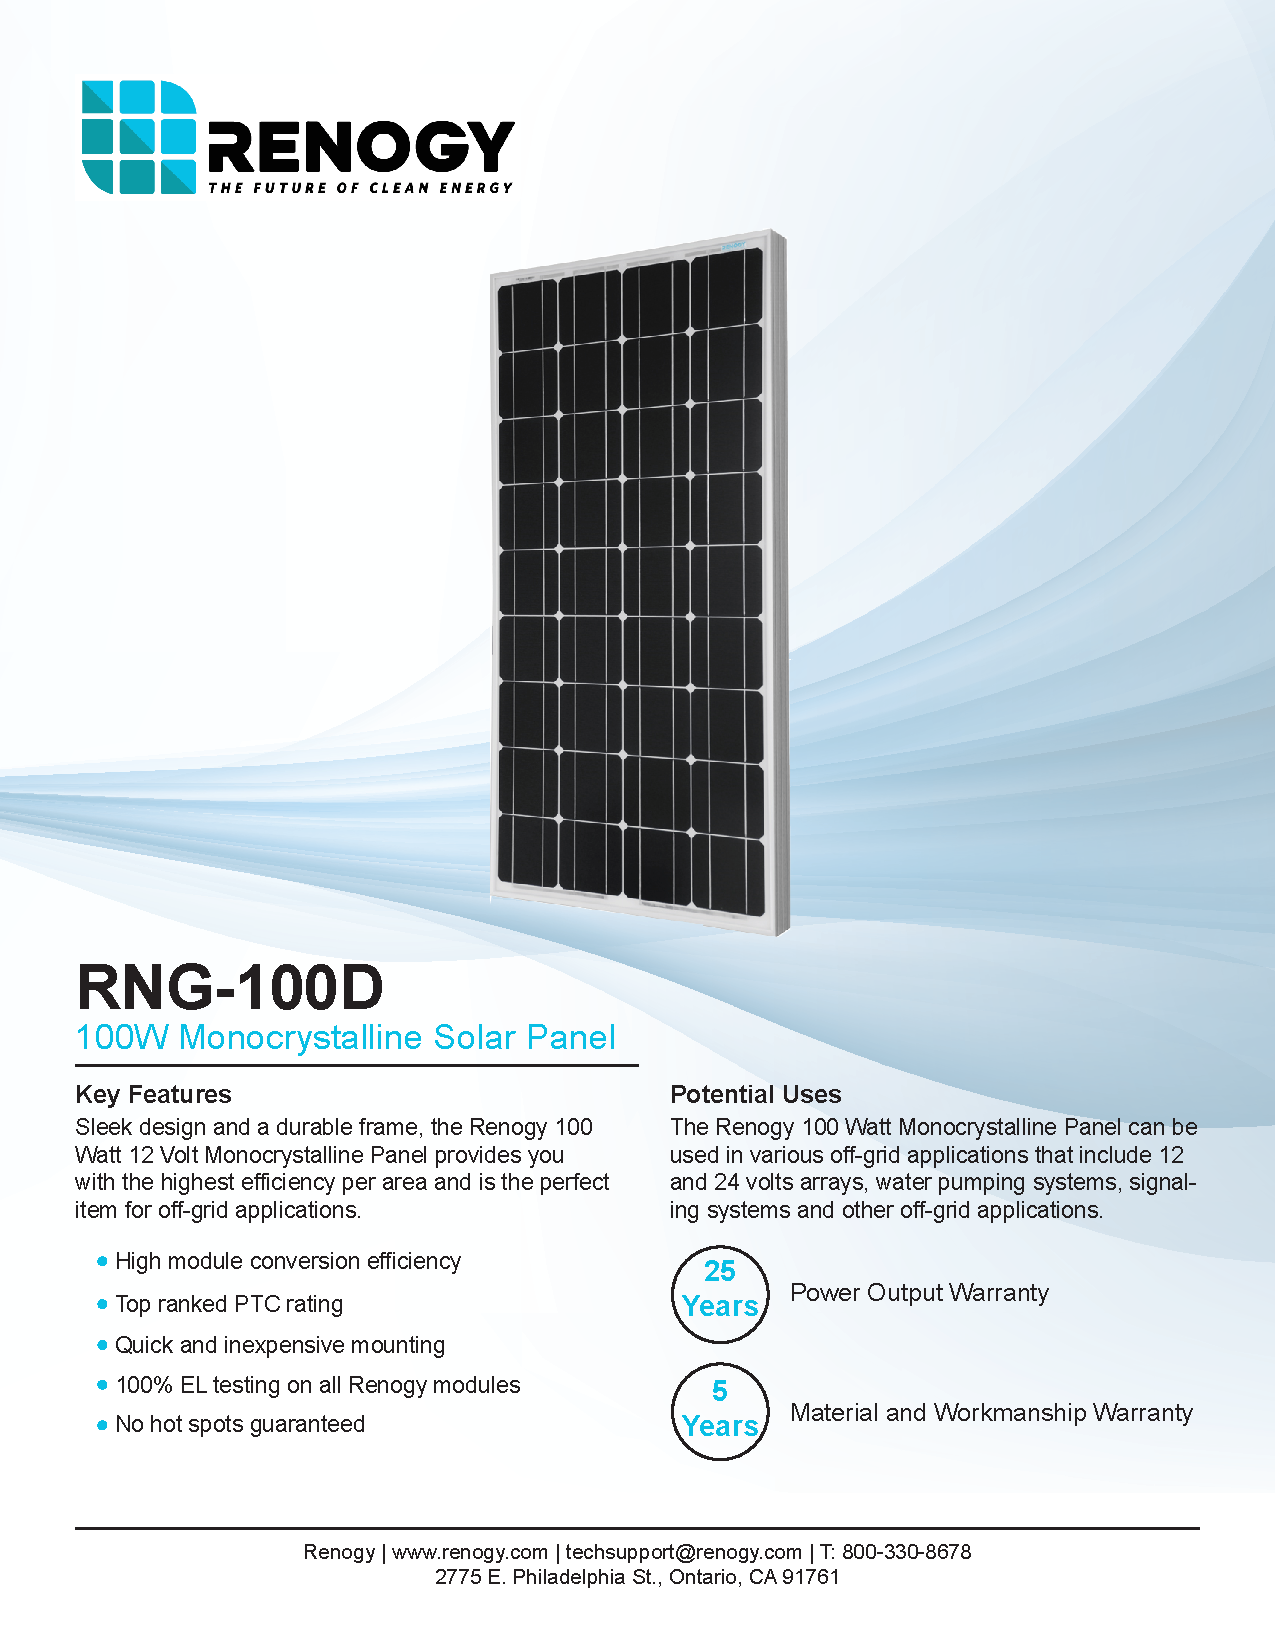
\includepdf[pages=-]{PDFs/100-Watt-12-Volt-Monocrystalline-Solar-Panel-Specifications}
    \includepdf[pages={1-4}]{PDFs/TerminalBlock}
    \includepdf[pages={1-3}]{PDFs/1N5400}
    \includepdf[]{PDFs/Resistence}
    \includepdf[pages={1-6}]{PDFs/TLP175A}
    \includepdf[pages={1-6}]{PDFs/1N4148}
    \includepdf[pages={1-4}]{PDFs/LYCA005x}
    \includepdf[pages={1-5}]{PDFs/2N2219}
    \includepdf[pages={1,3,4,5,7,8}]{PDFs/18650}
\end{document} 